\documentclass[10pt]{report}
\usepackage[margin=1in]{geometry}
\usepackage[utf8]{inputenc}
\usepackage[english]{babel}
\usepackage[T1]{fontenc}
\usepackage{fourier}
\usepackage{amsthm}
\usepackage{amssymb}
\usepackage{amsmath}
\usepackage{amsfonts}
\usepackage{latexsym}
\usepackage{graphicx}
\usepackage{float}
\usepackage{etoolbox}
\usepackage{hyperref}
\usepackage{tikz}
\usepackage{lipsum}


\newcommand{\R}{\mathbb{R}}
\newcommand{\N}{\mathbb{N}}
\newcommand{\Z}{\mathbb{Z}}
\newcommand{\Q}{\mathbb{Q}}
\newcommand{\C}{\mathbb{C}}


\title{Assignment I: The softmax function}
\author{Luca Lombardo}


\begin{document}
% \maketitle

% \tableofcontents

\setlength{\parindent}{0em}
\setlength{\parskip}{-0.5em}

\section*{Results}
This section presents a comparative analysis of three softmax function implementations under varying conditions. We evaluate the \texttt{softmax\_auto} implementation with and without the \texttt{parallel} directive and compare performance between AVX2 and AVX512 instruction sets.

\paragraph{Experimental Setup} All experiments were conducted on a system equipped with dual Intel(R) Xeon(R) Gold 5318Y CPUs, providing a total of 96 threads (48 per CPU). The system has 1TB of RAM and runs Ubuntu 22.04 with Linux kernel 5.15.0-119-generic. All code was compiled using GCC 11.4.0 with appropriate optimization flags.

\subsection*{Performance}

We compare the execution time of three softmax implementations across various input sizes, analyzing the effects of parallelization and vectorization instruction sets on the auto-vectorized implementation. Figures~\ref{fig:perf_noparallel_avx512} and \ref{fig:perf_noparallel_noavx512} demonstrate performance without parallelization, while Figures~\ref{fig:perf_parallel_avx512} and \ref{fig:perf_parallel_noavx512} show results with parallelization enabled.

\begin{figure}[H]
  \centering
  \begin{minipage}{0.49\textwidth}
    \centering
    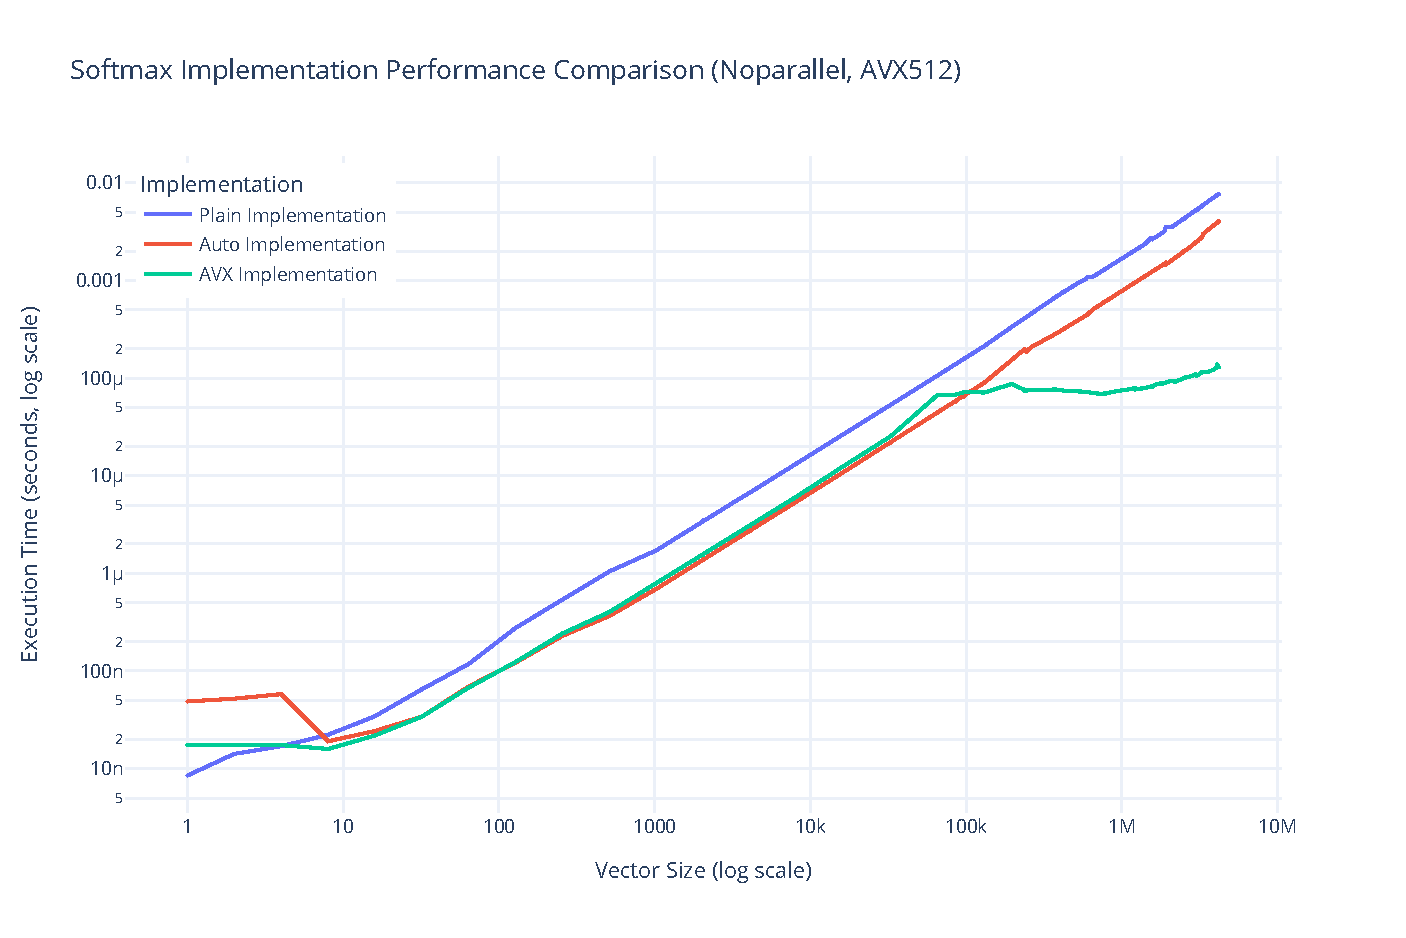
\includegraphics[width=\textwidth]{../images/performance/softmax_noparallel_avx512.pdf}
    \caption{Performance of softmax implementations without parallelization and with AVX512 instructions.}
    \label{fig:perf_noparallel_avx512}
  \end{minipage}
  \hfill
  \begin{minipage}{0.49\textwidth}
    \centering
    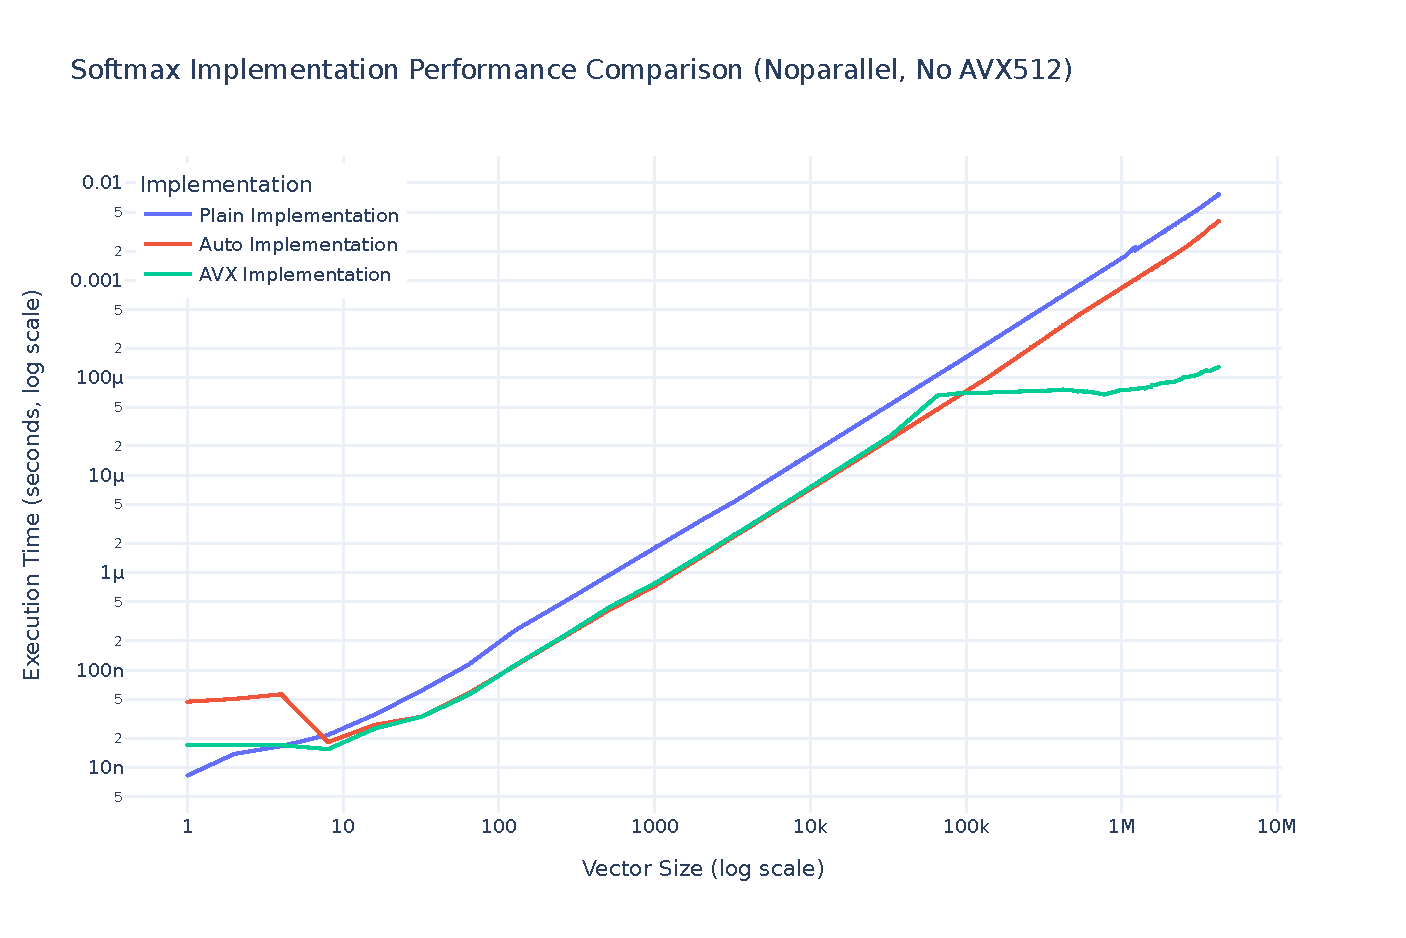
\includegraphics[width=\textwidth]{../images/performance/softmax_noparallel_noavx512.pdf}
    \caption{Performance of softmax implementations without parallelization and without AVX512 instructions.}
    \label{fig:perf_noparallel_noavx512}
  \end{minipage}
\end{figure}


\begin{figure}[H]
  \centering
  \begin{minipage}{0.49\textwidth}
    \centering
    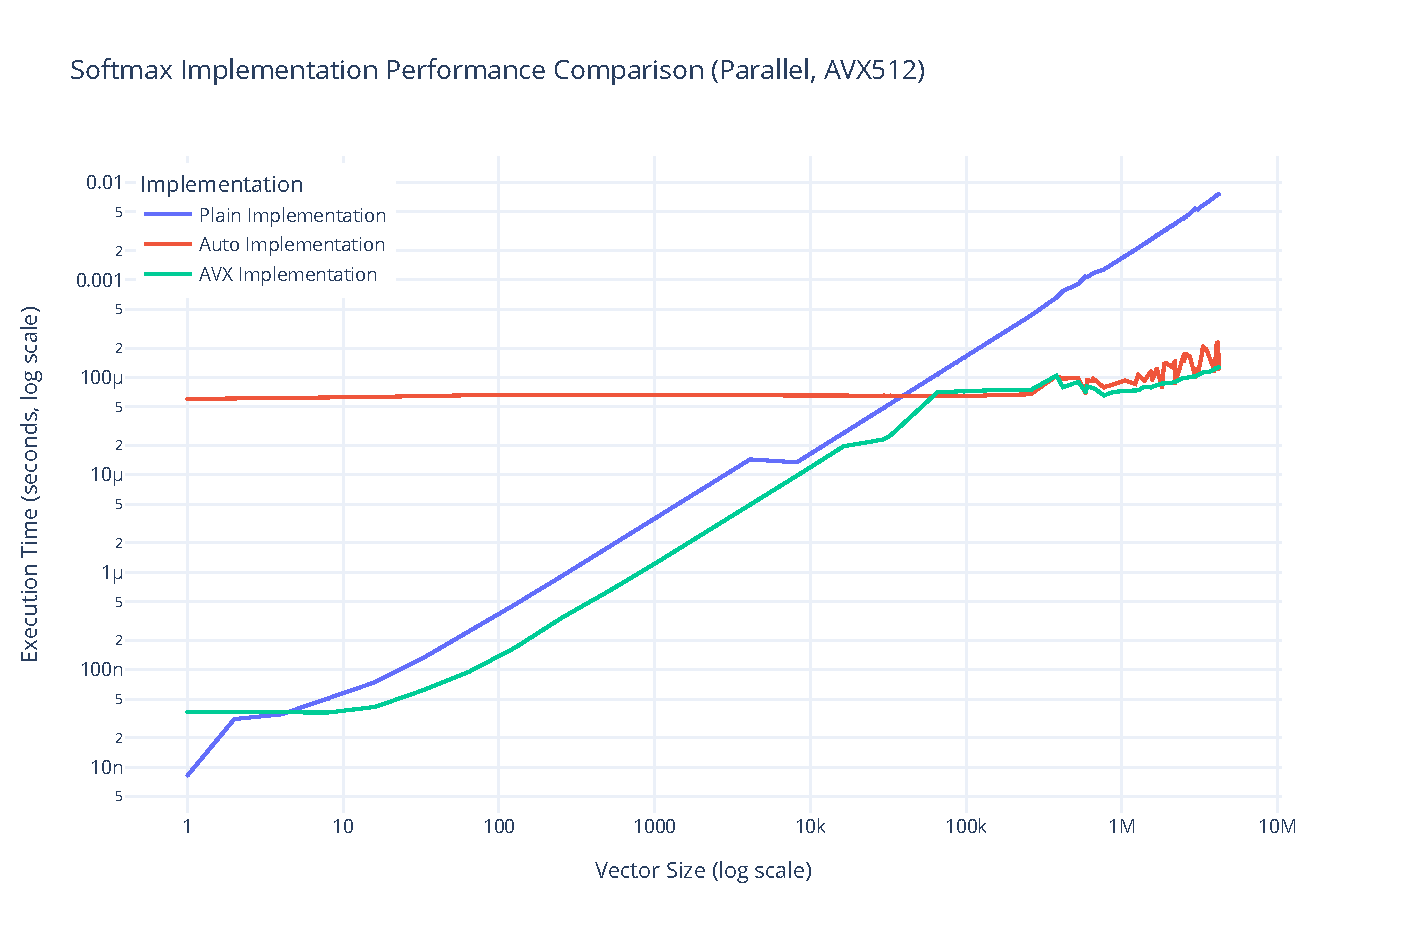
\includegraphics[width=\textwidth]{../images/performance/softmax_parallel_avx512.pdf}
    \caption{Performance of softmax implementations with parallelization and AVX512 instructions.}
    \label{fig:perf_parallel_avx512}
  \end{minipage}
  \hfill
  \begin{minipage}{0.49\textwidth}
    \centering
    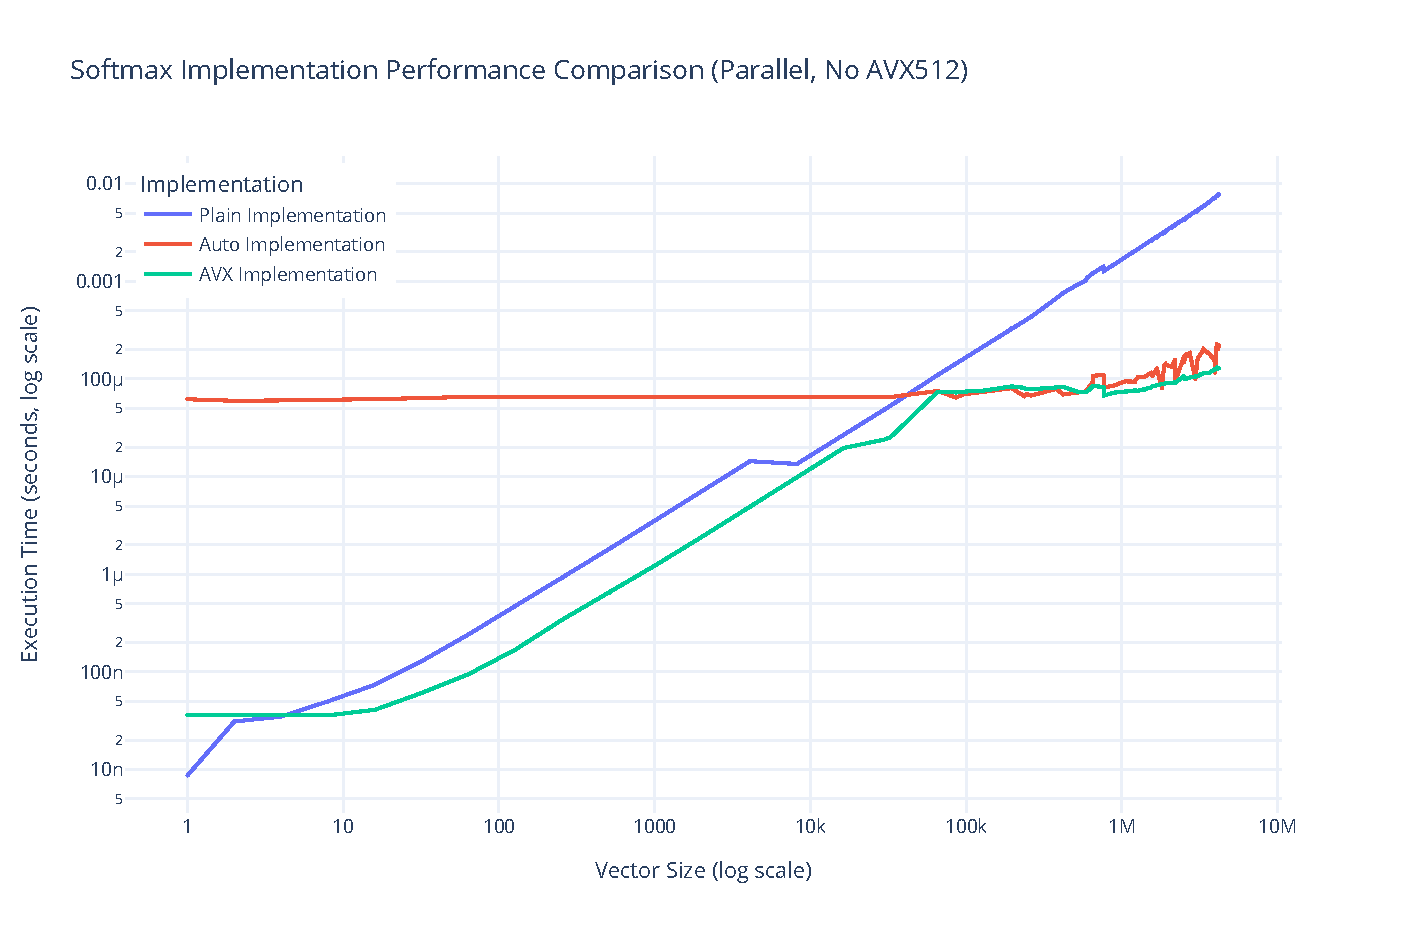
\includegraphics[width=\textwidth]{../images/performance/softmax_parallel_noavx512.pdf}
    \caption{Performance of softmax implementations with parallelization but without AVX512 instructions.}
    \label{fig:perf_parallel_noavx512}
  \end{minipage}
\end{figure}

The manually vectorized implementation \texttt{softmax\_avx} employs an optimization strategy where parallelization is deliberately not enabled for small input sizes (fitting within L1 cache) to avoid thread management overhead. As evidenced in the performance profiles, when the input size becomes larger, the manually vectorized implementation (that is parallelized) outperforms the auto-vectorized implementation (both with and without parallelization). It should be noted that the logarithmic scaling on both axes helps with visualization across multiple orders of magnitude but obscures less evident performance differentials between implementations. The following section will give a clearer visualization of the performance differences.

\subsection*{Speedup}
We analyze the relative speedup of various configurations compared to the baseline plain implementation. Figures~\ref{fig:speedup_parallel_avx512} through \ref{fig:speedup_noparallel_noavx512} illustrate the performance gains achieved through different combinations of parallelization and vectorization techniques.

\begin{figure}[H]
  \centering
  \begin{minipage}{0.49\textwidth}
    \centering
    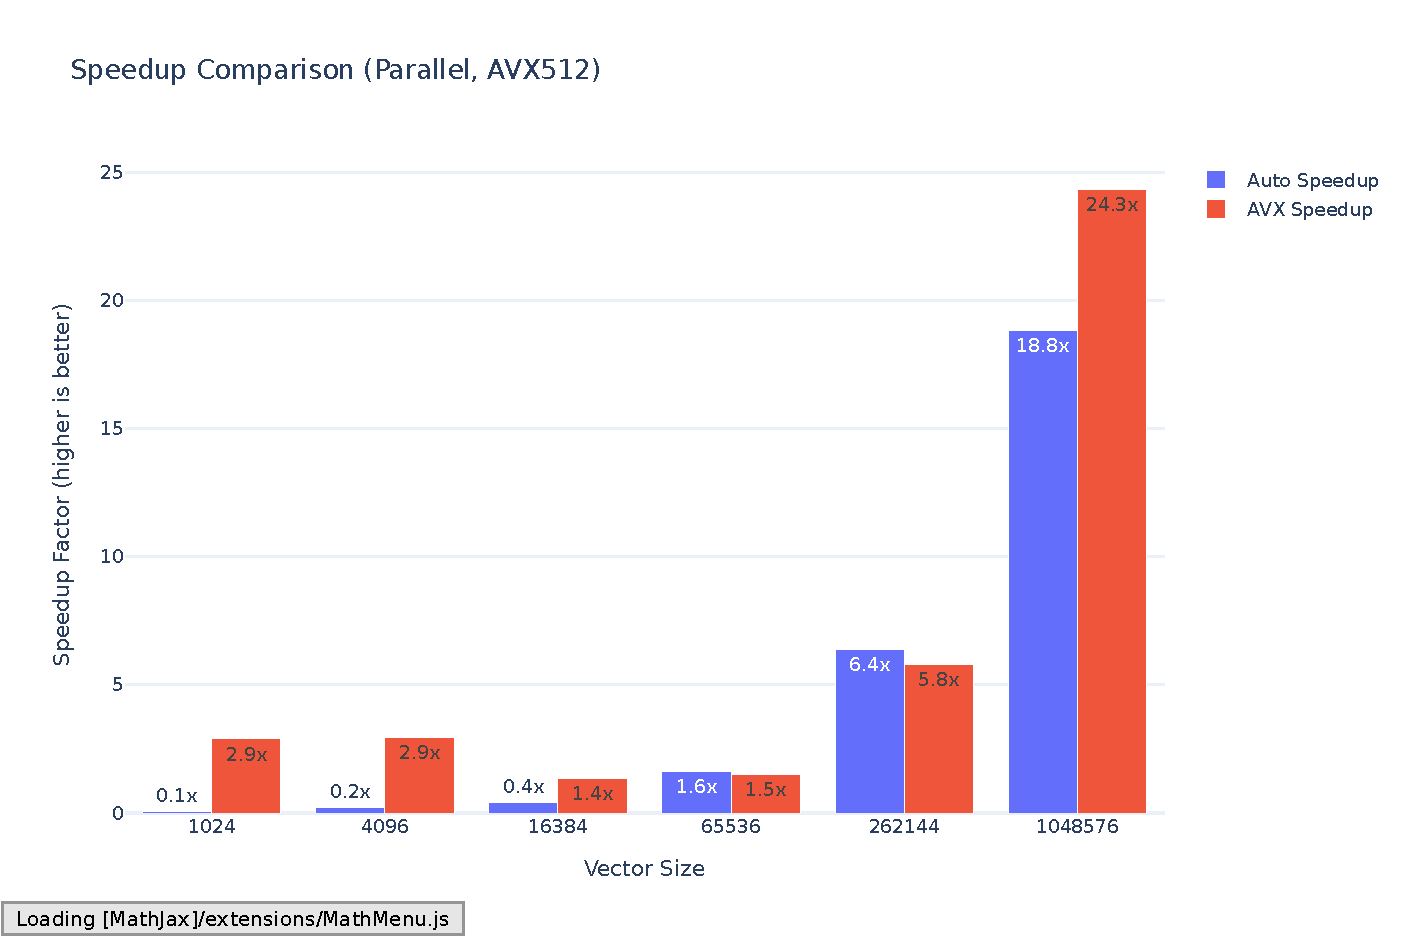
\includegraphics[width=\textwidth]{../images/speedup/softmax_speedup_parallel_avx512.pdf}
    \caption{Speedup with parallelization and AVX512 instructions.}
    \label{fig:speedup_parallel_avx512}
  \end{minipage}
  \hfill
  \begin{minipage}{0.49\textwidth}
    \centering
    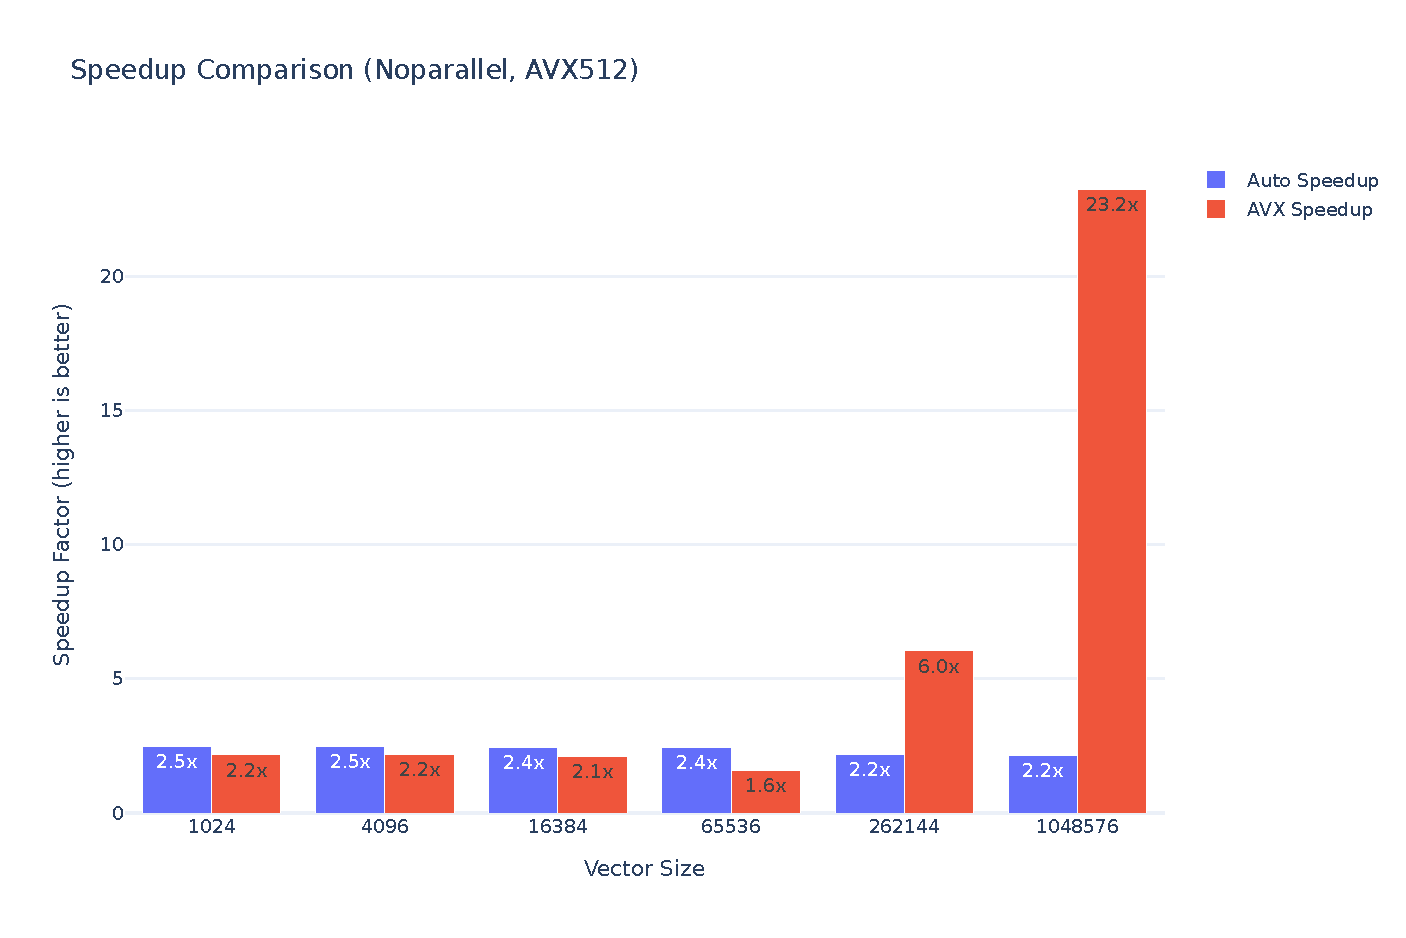
\includegraphics[width=\textwidth]{../images/speedup/softmax_speedup_noparallel_avx512.pdf}
    \caption{Speedup without parallelization but with AVX512 instructions.}
    \label{fig:speedup_noparallel_avx512}
  \end{minipage}
\end{figure}

\begin{figure}[H]
  \centering
  \begin{minipage}{0.49\textwidth}
    \centering
    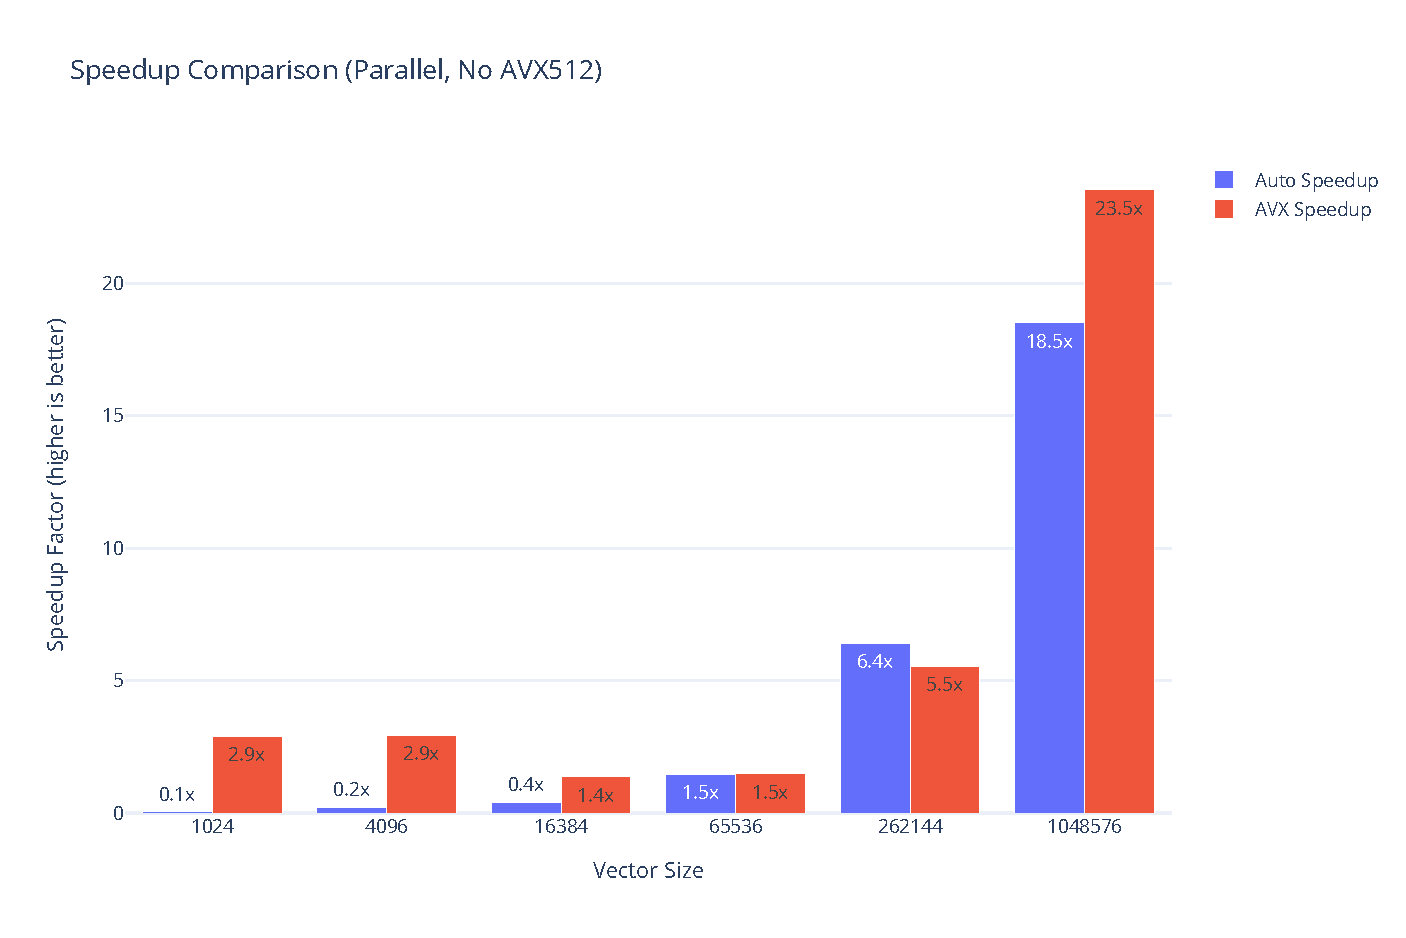
\includegraphics[width=\textwidth]{../images/speedup/softmax_speedup_parallel_noavx512.pdf}
    \caption{Speedup with parallelization but without AVX512 instructions.}
    \label{fig:speedup_parallel_noavx512}
  \end{minipage}
  \hfill
  \begin{minipage}{0.49\textwidth}
    \centering
    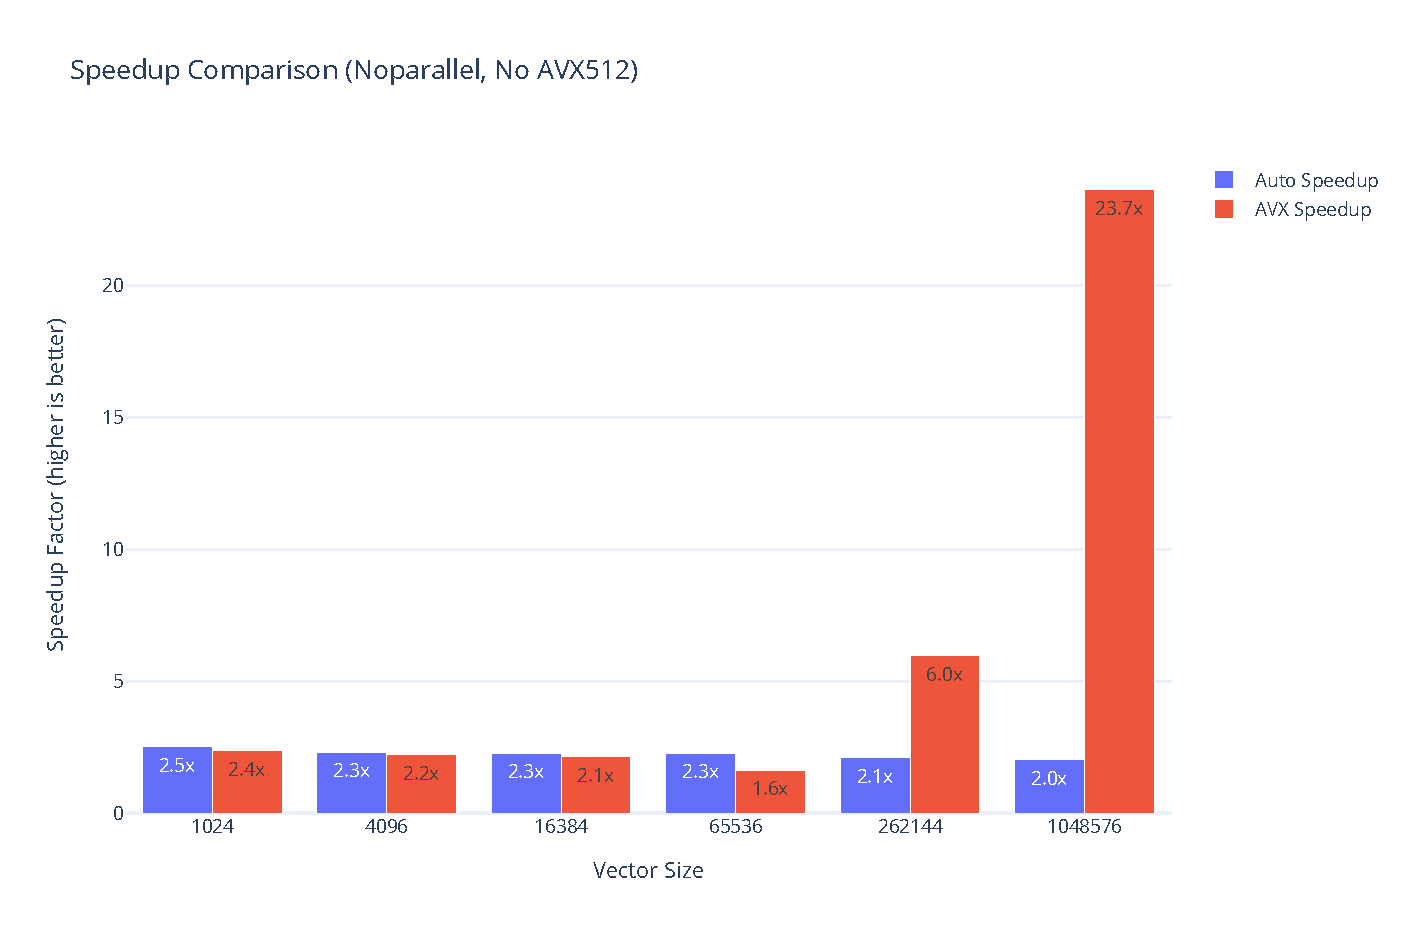
\includegraphics[width=\textwidth]{../images/speedup/softmax_speedup_noparallel_noavx512.pdf}
    \caption{Speedup without parallelization and without AVX512 instructions.}
    \label{fig:speedup_noparallel_noavx512}
  \end{minipage}
\end{figure}

Figures~\ref{fig:speedup_parallel_avx512} and \ref{fig:speedup_parallel_noavx512} demonstrate that parallelization yields substantial performance benefits for the auto-vectorized implementation with large input dimensions, while introducing counterproductive overhead for smaller inputs, reducing efficiency to levels comparable with scalar implementation. Regarding instruction set influence, comparative analysis between Figures~\ref{fig:speedup_parallel_avx512} and \ref{fig:speedup_parallel_noavx512}, as well as between Figures~\ref{fig:speedup_noparallel_avx512} and \ref{fig:speedup_noparallel_noavx512}, indicates that AVX512 provides marginal performance improvements over AVX2, with improvements coefficients remaining closely above statistical significance\footnote{I am very surprised by this result, as I expected a more significant performance boost from AVX512. I even looked at the disassembly code generated by the compiler to verify that the AVX512 instructions were indeed being used.}

\subsection*{Scalability}

We evaluate thread scalability using a fixed input size ($K = 2^{30}$) while varying thread count from 1 to 96. Figure~\ref{fig:thread_scaling} shows the execution times, while Figure~\ref{fig:thread_speedup} presents the speedup alongside the theoretical Amdahl's Law prediction. Notably, a performance discontinuity occurs at approximately half the maximum thread count, corresponding to the number of cores in one of the system's two physical processors.

\begin{figure}[H]
  \centering
  \begin{minipage}{0.49\textwidth}
    \centering
    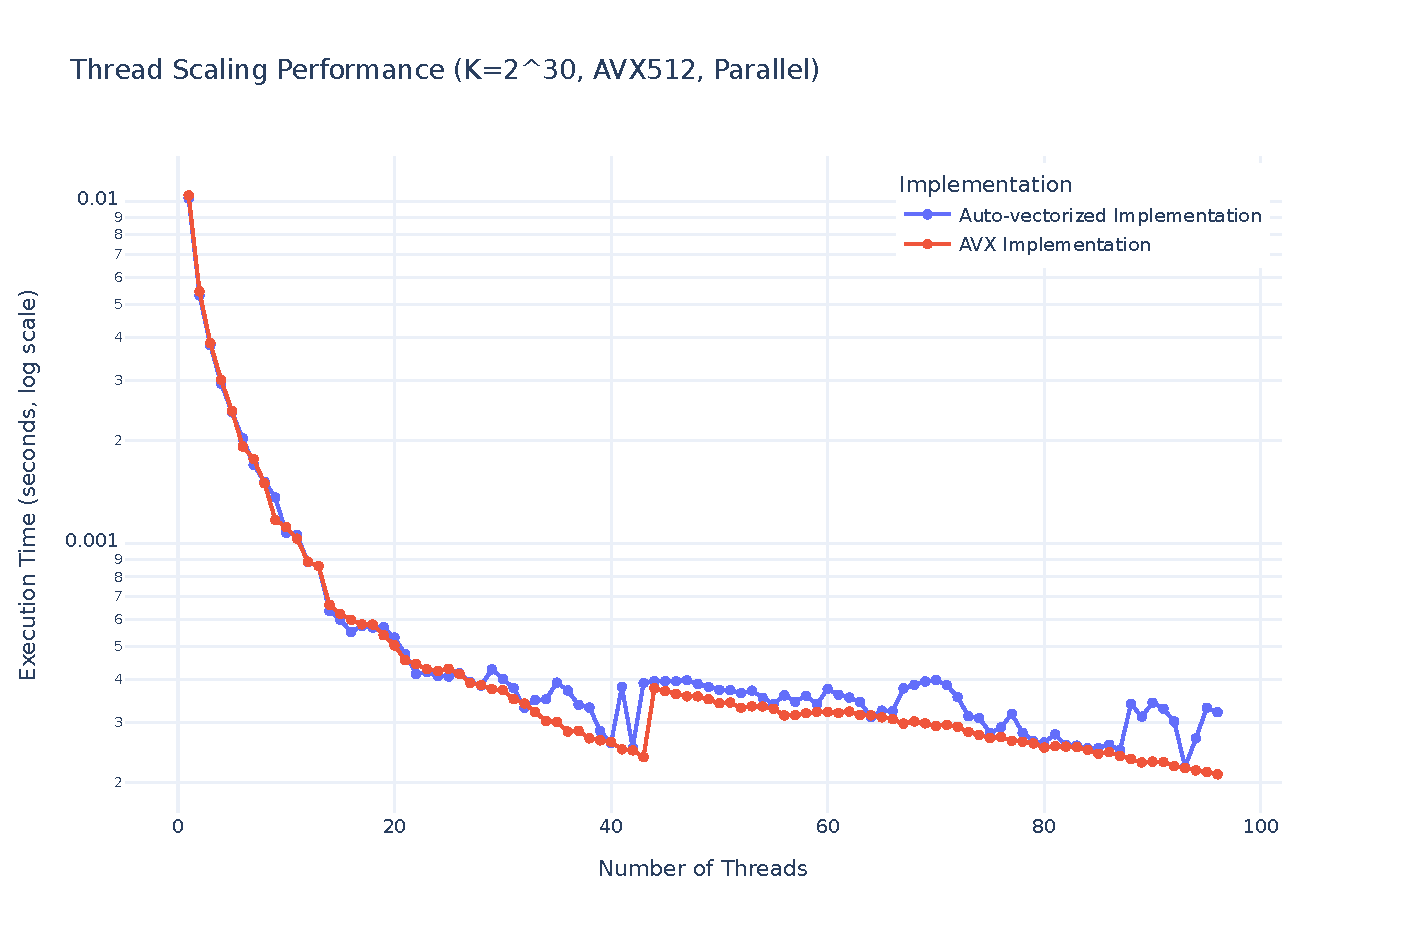
\includegraphics[width=\textwidth]{../images/thread_scaling/thread_scaling_avx512.pdf}
    \caption{Execution time scaling with thread count for the softmax implementations.}
    \label{fig:thread_scaling}
  \end{minipage}
  \hfill
  \begin{minipage}{0.49\textwidth}
    \centering
    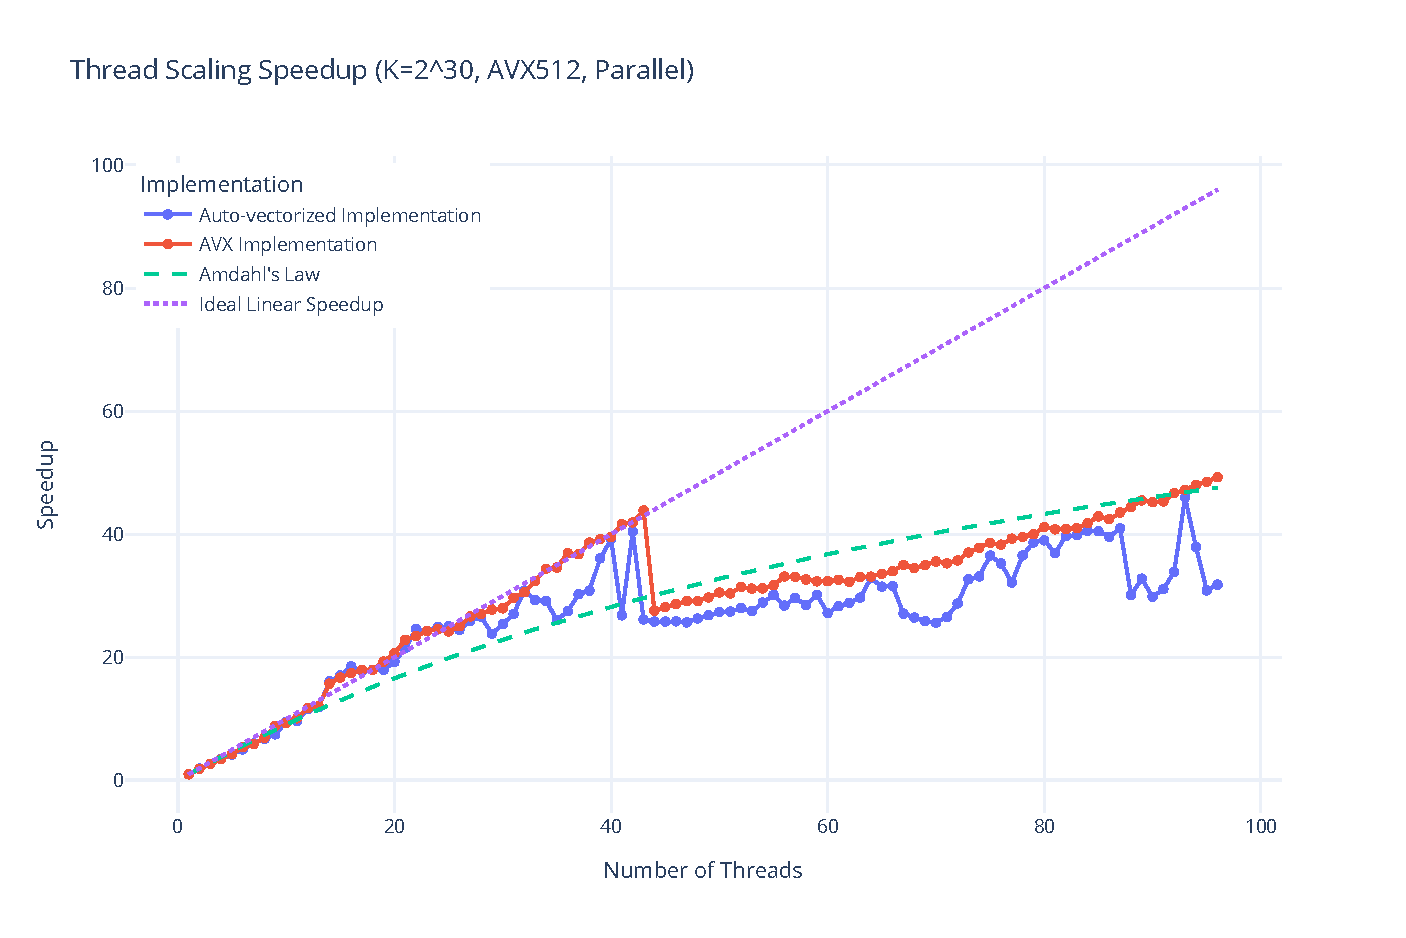
\includegraphics[width=\textwidth]{../images/thread_scaling/thread_scaling_speedup_avx512.pdf}
    \caption{Thread scaling speedup compared to Amdahl's Law prediction.}
    \label{fig:thread_speedup}
  \end{minipage}
\end{figure}

\subsection*{Numerical Stability}
We evaluate numerical stability by measuring how closely the sum of each implementation's output approximates the theoretical value of 1.0. Figure \ref{fig:stability_1M} demonstrates that the plain implementation shows numerical instability at moderate dimensions ($K = 2^{20}$), while both vectorized implementations maintain stability. Figure \ref{fig:stability_1B}, which excludes the significantly divergent plain implementation for clarity, reveals that the manually vectorized implementation achieves superior numerical precision compared to the auto-vectorized variant at very large dimensions. Nevertheless, the auto-vectorized implementation maintains acceptable numerical stability even at substantial input sizes ($K=2^{30}$). The superior numerical stability of \texttt{softmax\_avx} can be attributed to several implementation factors: its controlled horizontal reduction pattern, block-based processing that limits error propagation, precise handling of non-aligned elements through explicit masking, and deterministic operation ordering. In contrast, \texttt{softmax\_auto} relies on compiler-determined reduction strategies and lacks the explicit error-controlling mechanisms of the manually vectorized implementation.

\begin{figure}[H]
  \centering
  \begin{minipage}{0.49\textwidth}
    \centering
    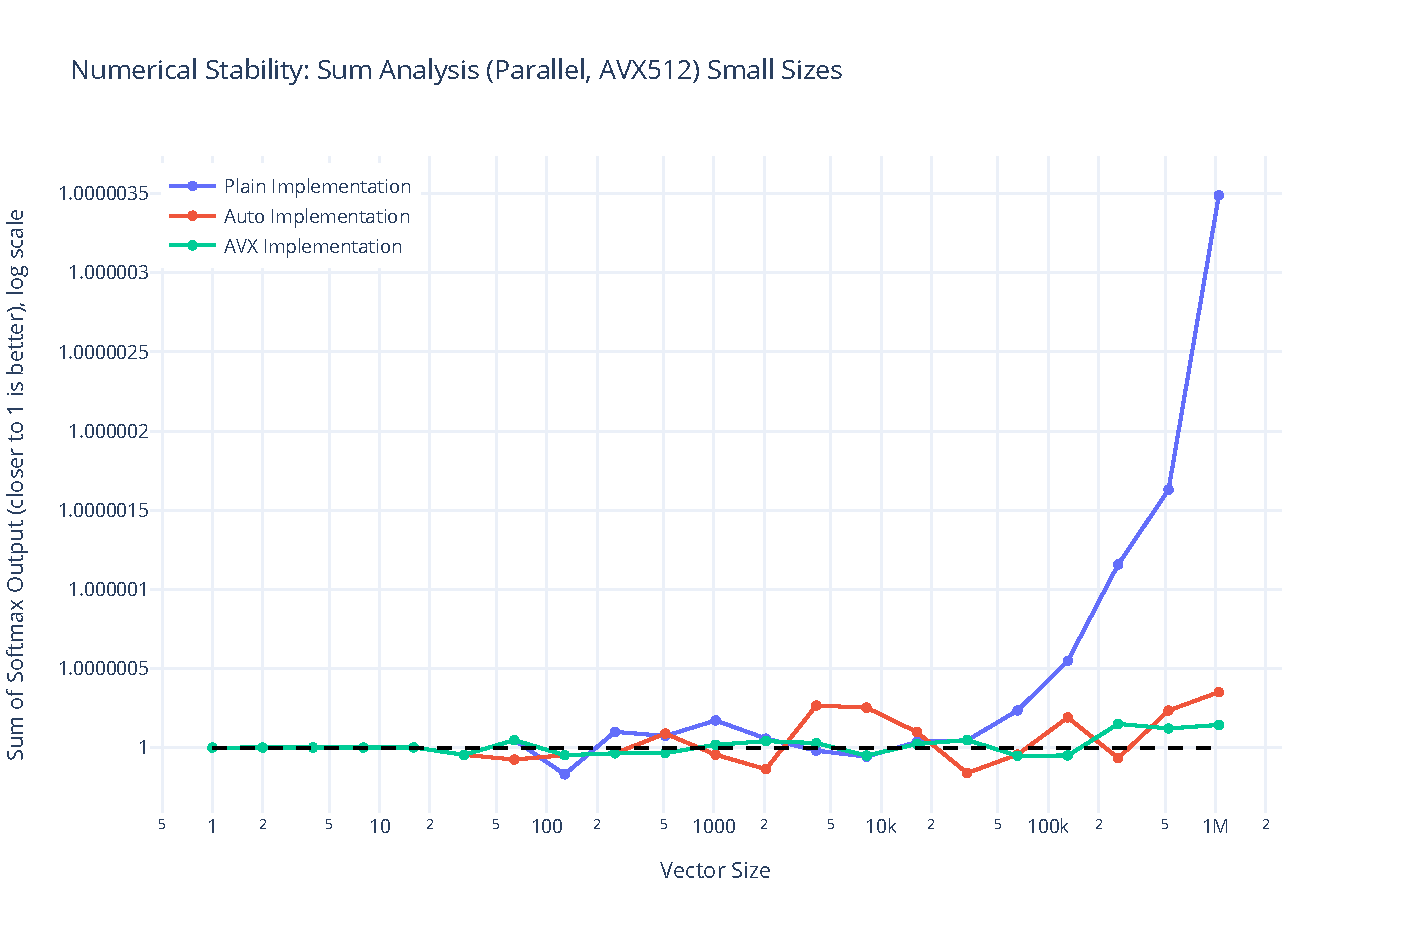
\includegraphics[width=\textwidth]{../images/stability/stability_parallel_avx512_1M.pdf}
    \caption{Numerical stability with small input sizes.}
    \label{fig:stability_1M}
  \end{minipage}
  \hfill
  \begin{minipage}{0.49\textwidth}
    \centering
    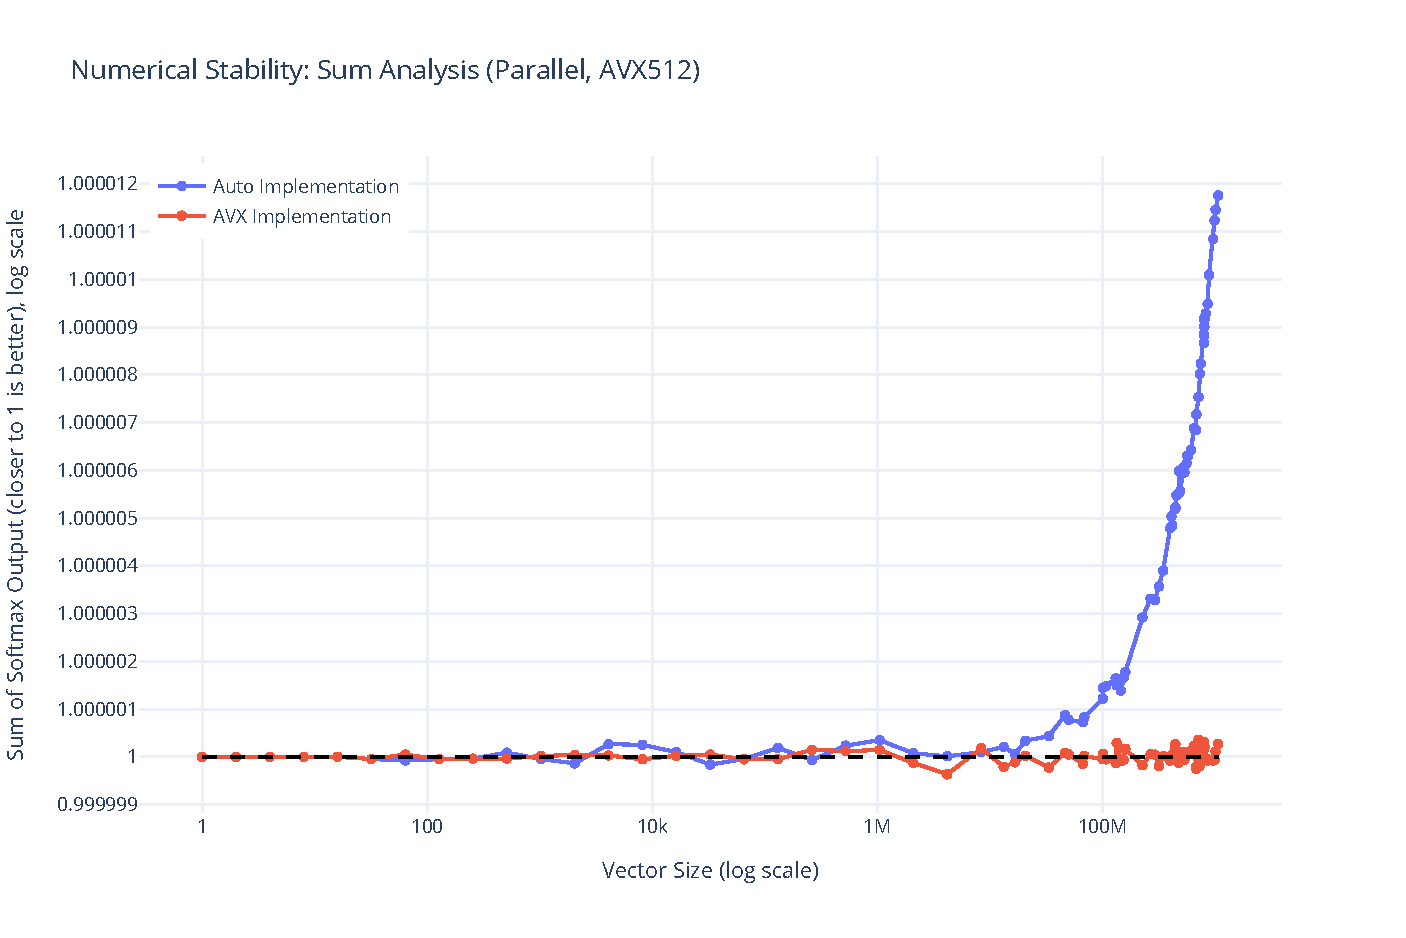
\includegraphics[width=\textwidth]{../images/stability/stability_parallel_avx512_1B.pdf}
    \caption{Numerical stability without large input sizes.}
    \label{fig:stability_1B}
  \end{minipage}
\end{figure}

\end{document}
